\chapter{Case study}

The methodology for this master's thesis will be divided into four distinct stages to achieve the goals of the study. The first step will involve an analysis of the current low voltage grid in the rural area of western Germany, including a review of the existing grid structure, load distribution, and grid components. The second stage will be the future load forecast, which will estimate the expected load on the grid resulting from the integration of electric vehicles (BEVs) and heat pumps. This will be accomplished through the comparison of data from relevant sources, including Fraunhofer Institut and when2heat~\cite{when2heat}, but also the utilising simulation tools such as UrbanHeatPro~\cite{urbanheatpro}, emobpy~\cite{emobpy}.  The third stage will be the modelling of the future grid to assess the impact of e-mobility and heat pump integration on the network, utilising simulation tools, such as PowerFactory. The final stage will involve simulating different scenarios for grid reinforcements to identify potential solutions for improving the functionality and reliability of the network, including different calculation cases and variants. 

\section{Analysis of the current grid}

In order to analyse the current grid, load flow analysis to determine the distribution of power in the network and identify areas of congestion, while also analysing voltage stability to ensure voltage levels meeting standards at all points in the network. A short-circuit calculations is also done to determine fault current levels and select suitable protective devices in case of faults.

The actual grid is a low voltage grid of a small town in western Germany, presented in Fig. \ref{fig:grid}. The grid is a meshed low voltage grid of 0.4~kV with three 2-winding transformers. Transformer TR1 has a rating of 630~kVA, while the two other transformers, TR2 and TR3, have a rating of 250~kVA. Each transformer is attached to its corresponding external medium voltage grid of 20~kV. Additionally, the grid consists of 569 low voltage nodes, connected by 579 branches with 3 load buses. Along the lines, 342 general loads are attached. The highest active power of the general loads is at 145.4 kW and the lowest at 18 kW, with a power average of 31.7 kW. The layout of the diagram representing the low voltage grid is modified to keep anonymity and enhance the appearance. 

\begin{figure}[h]
    \centering
    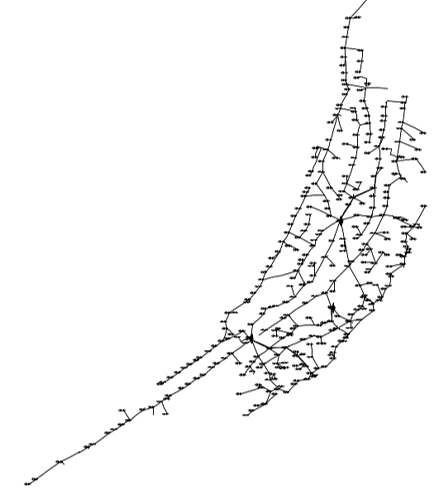
\includegraphics[scale=0.7]{thesis-latex/img/gridbase.png}
    \caption{Schematic representation of the current grid}
    \label{fig:grid}
\end{figure}

The active and reactive power from the loads is provided as steady-state average from empirical data of that area. The nominal frequency of the supply voltage shall be 50
Hz but frequency is set from the transmission system, so it is
not evaluated in this paper because of its small role for LV
systems with synchronous connection. It is important to
evaluate frequency in LV systems with no synchronous
connection when the power source operates in an island mode. %https://ieeexplore.ieee.org/stamp/stamp.jsp?tp=&arnumber=7161058

During this project a tool named Power Factory (PF) is applied. Developed by DigiSilent, the tool can analyse electrical energy supply for transmission, distribution, generation and industrial networks as well as for renewable energy systems. This program allows users to calculate load-flow, short-circuit and several other methods important for energy supply analysis.~\cite{noauthor_powerfactory_nodate}

\section{Electric load forecast}

As the first phase of the thesis, the future electric load in the grid must be developed. Due to the high increase of electrification, the future load for heat pumps and electric vehicle were calculated. Even though in future there might be an increase of households in the area, the isolation level of these house will be relatively low compared to the other houses that the impact is neglected in this thesis. The regular power consumption for each general load is also assumed not to vary in the future. 

\subsection{Heat pumps}
 
% simultaneity factor
In order to get realistic value of the heat pump load, the heat demand of the chosen grid had to be calculated first. The tool UrbanHeatPro was implemented to calculate the yearly heat demand with a 10-min resolution for each building in the grid~\cite{urbanheatpro}. As shown in Table \ref{tab:urbanheat}, in this tool 9 parameters are necessary to insert in the following order for each building in order to calculate the demand. The first parameter "bid" defines the building ID, which is different for each house, whereas the spatial area of the building is defined as "area". The area was found by using a free map calculation tool, which measures the acreage of a plot~\cite{maparea}. If a building was not represented in that area, an average area value of 103.6 m$^2$ was implemented~\cite{area}. "use" describes the type of building use, which defines if the building is residential, commercial, industrial or public. These values were found by using information in Google Maps~\cite{google}. "free\_wall" describes the amount of outside walls that are in contact with the ambient temperature. Here, all the buildings are assumed to be of rectangular form with four walls. The "year\_class" parameter describes the construction year of the building, while the "size\_class" describes the building type, which is either a single-family house (SFH), multi-family house (MFH), terraced house (TH) or an apartment block (AB). These two parameters were found by using the Geospin tool~\cite{geospin}. Additionally, the latitudinal and longitudinal coordinates for each building must be inserted and the distance from the heat source to the building is defined, which will be 0 in this case study, since only heat pumps are considered, which are directly installed inside of the building. 

\begin{table}[h]
    \centering
    \caption{Necessary input values for UrbanHeatPro}
    \begin{tabular}{|c|c|c|c|c|c|c|c|c|}
    \hline
        bid & area & use & free\_walls & year\_class & size\_class & lat & lon & dist2hp \\
        \hline
    \end{tabular}
    \label{tab:urbanheat}
\end{table}

Optional to those variables, the refurbishment level and number of occupants can be defined. However, due to the lack of sources regarding these parameters, approximated values are defined by considering the other already mentioned parameters and the TABULA topology tool~\cite{tabula}. The ambient temperature for this region is derived from the German weather service and ranges between -10°C to 31°C over the year~\cite{dwd}.

After calculating the heat demand from UrbanHeatPro, the heat pump electricity demand was calculated by dividing the hourly COP factor from when2heat depending on the desired heat pump technology~\cite{when2heat}. In this project, it was assumed that no house has floor heating and all building use radiator heating. 

In order to know the appropriate heat pump technology for each building, the heat pump traffic light from Ffe was analysed~\cite{wpampel}. With this tool, the building's distance to other buildings and green area is investigated to know if it is technically possible to install a heat pump. The traffic light project investigates ASHP, GSHP, GWHP and a heat pump with solar heating and ice storage. The possibility of having a heat pump is defined as definite, possibly or not possible, whereas possibly describes that more detailed measurements are necessary in order to make a secure decision. The latter will not be taken into account in this thesis, since it is assumed that most consumers will rather prefer installing a ASHP or GSHP like stated in section \ref{sec:markethp}. All buildings having the definite option to install a ASHP will be having a ASHP load profile in the PowerFactory simulation, while the buildings not or possibly having the possibility of ASHP but have a definite possibility of having a GSHP will have a GSHP load profile. Due to its energy efficient properties, the GWHP is assumed to not have a high impact on the grid and will therefore not be taken into account in the standard simulation. Considering the information mentioned above, 56\% of all buildings in the area have a definite possibility of installing a heat pump.

EU Richtlinien -> Hausstandard (auch bei UrbanHeatPro)
Three load profiles for HP will exist depending on different energy efficiency standards with maximums of 100 kWh/(m$^2$a), 160 kWh/(m$^2$a) and 200 kWh/(m$^2$a). The higher energy standards will not be considered, since the EU commission decided that all houses with a lower standard have to be improved by a maximum of 200 kWh/(m$^2$a) by 2030 for all residential buildings and by 160 kWh/(m$^2$a) by 2033~\cite{EPBD_2021}.

\subsection{Electric vehicle}

The electric vehicle load profile is defined by the emobpy tool~\cite{emobpy}. Emobpy is an open tool which creates battery electric vehicle power consumption in time-series based on empirical data. Three types of drivers are generated: commuter full time (CFT), commuter part time (CPT) and non-commuter full time (NFT). The commuters leave the residence to go to work and come back after work, representing a full time or part time worker. On the other hand, the non-commuter full time does care work and represents stay-at-home mothers and fathers. Based on \cite{labourforce}, the ratio of the type of driver is defined as 48\% for CFT, 14\% for CPT and 38\% for NFT. Additionally to this input, the amounts of trip per day, distance and duration per trip, departure time and destination per trip, maximal/minimal time at the location and overall location per day is defined by \cite{mid} and illustrated in appendix \cite{sec:inputemobpy}. As a second step the vehicle details must be determined. The representative cars for this simulation are the Model 3 Tesla and the Kona Hyundai since these models have one of the largest market shares in Germany~\cite{kbaneuzulassung}. The road condition is set to good quality and having none to low slope gradient. The charging station availability is defined by probabilities depending on the station and are represented in Table \ref{tab:probcharg}. Depending on the purpose of the trip, the probability of the charging availability and charging capacity varies. For instance, a person that drives to work has 50\% chance of charging with 11~kW and a 25\% chance of charging with 22~kW. On the other side, a person driving long distance will only have a 1\% chance of fast charging and no other possibilities. 

\begin{table}[h]
    \centering
    \caption{Charging station availability of emobpy for a fulltime commuter}
    \begin{tabular}{|c|c|c|c|}
    \hline
        \textbf{Purpose} & \textbf{11~kW} & \textbf{22~kW} & \textbf{Fast charging} \\
        \hline
        Errands & 0 & 0.5 & 0  \\ 
        Escort & 0 & 0.5 & 0  \\
        Leisure & 0 & 0.5 & 0  \\
        Shopping & 0 & 0.5 & 0  \\
        Home & 1 & 0 & 0 \\
        Workplace & 0.5 & 0.25 & 0 \\
        Driving & 0 & 0 & 0.01 \\
        \hline
    \end{tabular}
    \label{tab:probcharg}
\end{table}

As the last step, a charging strategy must be chosen. In this simulation, the immediate at full capacity strategy is used, which means that the BEV charge their batteries at full power rating as soon as they arrive at charging stations. The charging stops when the battery is full, or when the next trip starts. Based on \cite{geospin}, the fast charging potential in the analysed area is relatively small with 3.2-4.9 public charging hours per day. Hence the attraction for charging point operators is small.  

%simultaneity factor ffn studie
% When developing the simultaneity factor regarding BEV, the average daily route, specific energy consumption of the car, charging power, charging behaviour and size of the vehicle must be considered. 


\section{Modelling of the future grid}

As the third phase of the project, the future grid is modeled. Several realistic scenarios are developed for the year 2030 and 2045. These yars are used as benchmarks due to the Germans governments climate goals for 2030 and 2045~\cite{bmwk2022}. These scenarios are then being simulated with the corresponding load profiles of the heat pumps and electric vehicles developed in phase one. The expected outcome of this phase is to discover the upcoming weaknesses and strength in the grid depending on the scenario.

Houses will have a simultaneity factor of 0.6, EV of goes up to 0.15 and in winter HP goes up to 1. %https://www.consentec.de/wp-content/uploads/2020/12/PDF_et_12_2020_S.41-44.pdf


\subsection{Scenarios}

In order to achieve realistic goals in the project, different possible scenario outcomes must be decided. Germany has pledged to reduce greenhouse gas emission in 2030 by 65\% compared to 1990 and to be fully climate neutral by 2045 in order to take on global warming~\cite{bmwk2022}. Hence 2030 and 2045 will be the benchmark years in this project. The proposed scenarios consider different cases ranging from a highly low electrification effort scenario to a high effort scenario. Additionally, for each scenario the grid will be analysed in three cases: only HP, only EV and HP+EV in order to integrate a sensitivity analysis. 

To develop realistic and independent scenarios, the method of scenario development defined by the Bergische Universität Wuppertal is applied~\cite{Planung}. Part of the scenario development is to estimate the future electricity demand regarding different evolution. The scope of the scenarios was found by applying the number of HPs and EVs listed in the Netzentwicklungsplan for 2037 and 2045~\cite{netzentwicklungsplan}. To get the estimated number of 2030, an interpolation between 2022 and 2037 was done. To achieve a ratio for the local grid, the future trend of the growth in housing and cars is calculated. Hence the scenario ratio is displayed in Table \ref{tab:scenario}.

\begin{table}[h]
    \centering
    \caption{Development of the scenarios}
    \begin{tabular}{c|cc|cc|}
    \cline{2-5}
         & \multicolumn{2}{c|}{Heat pumps} & \multicolumn{2}{c|}{Electric vehicles}\\
         & 2030 & 2045 & 2030 & 2045 \\
        \hline
        \multicolumn{1}{|c|}{Scenario A} & 10\%& 25\%& 29\% & 67\%\\
         \multicolumn{1}{|c|}{Scenario B} & 12\%&33\%&33\%&71\% \\
          \multicolumn{1}{|c|}{Scenario C} & 14\%&53\%&36\%&71\% \\
          \hline
    \end{tabular}
    \label{tab:scenario}
\end{table}

Scenario A is the low electrification effort scenario. In this future, hydrogen is the main energy carrier of the end-consumer and electricity is only used in applications we use today, for instance light or electronic appliances. Scenario B is the medium electrification effort scenario. Here electricity is used in more applications than today, for instance industrial heat processes or chemical processes. In scenario C, the electrification effort is the highest. This future has the same end transformation than B, but a faster and more efficient transition. 

        
%Assumptions and restrictions
The increase of households and buildings, or demographic change in the area is not taken into account. Additionally only home or work charging with respectively 11~kW or 22~kW are considered during the simulation. On household is also assumed to only have one car. In rural areas more than 60\% of the households only have one car~\cite{VDEFNN_2021}.


\subsection{Sensitivity analysis of input values}

A sensitivity analysis of the heat pumps and the electric vehicle loads is calculated as well, where the values of the inputs vary and the impact on the output is observed, to determine which inputs have the most significant impact. The input values are to compare the heat pump technologies: ASHP, GSHP, and GWHP with each other, but also compare the impact importance of heat pumps compared to electric vehicles. 

The sensitivity analysis can help to identify which inputs are the most critical to the model outcome, and provide insight into the robustness of the model. 


\section{Grid reinforcement}

The last and fourth phase of the thesis is the grid reinforcement strategies and the economic assessment, where options of grid reinforcements are compared in a technical and economical manner.  

\subsection{NOXVA principle}

The abbreviation NOXVA stands for "Network Optimisation before Flexibility utilisation before Reinforcement before Expansion" and is a further development of the NOVA principle ("Network Optimisation before Reinforcement and Expansion"). Accordingly, the current network operation should first be optimised (e.g. reactive power control, switch state). Then, flexibility is used, such as active and reactive power from generation plants, consumers and storage. The intervention in the market to maintain network security, such as peak shaving of end-consumers, should only be a last resort. If network congestion continues to occur, operating resources are reinforced. Eventually, if these combined measures are not enough to avoid network congestion, conventional network expansion takes place. The NOXVA principle is based on a natural order to minimise economic costs. This means that first, the measures are causing the lowest costs are implemented and only if these are not sufficient, the more expensive network expansion takes place.~\cite{noxva} 

\subsection{MONA principle}
%https://www.ffe.de/veroeffentlichungen/projekt-mona-2030-abschlussbericht-einsatzreihenfolgen-veroeffentlicht/

The "Merit-Order Netz-Ausbau 2030" (MONA 2030) principle analysed the necessary change in the grid infrastructure and compared these measures and technologies regarding grid optimisation in transmission and distribution networks. The cost-optimal order of expansion and installation of grid reinforcement possibilities is defined in order to develop a structured and standardised process.~\cite{mona}

Depending on the current problematic in the grid, different measures must be taken into account regarding MONA 2030. The techno-economic evaluation of network optimisation measures shows that regarding voltage stability, especially the measures of grid-optimising operations (peak shaving, reactive power management and TSH) both technically and from an overall cost perspective present the best alternative. The grid-oriented measures also point to financial benefits in the future, due to falling costs for ICT and battery prices, but their technical potential for reducing voltage violations is small. In general, however, it can be stated that in the case of voltage stability, all grid reinforcements have a positive effect, albeit in some cases, especially with self-consumption-optimised charging controls, the difference is very low. The rONT and LVR are more expensive than the other measures, similar to conventional grid expansion, but offer higher technical efficiency reducing voltage violations.~\cite{mona} 

Regarding equipment overloads, a smaller number of grid-optimisation operations have a better effect on the grid than with voltage stability. Measures such as reactive power control rather a negative effect on overloading. Apart from transformer replacement, only peak shaving has a potential to reduce the overloading of equipment, which can be leveraged at low cost.~\cite{mona}

\subsection{Priority of reinforcement}

Considering these two principles, below the priority used in the reinforcement strategy are defined. For every category, the measures are listed depending on their cost-effectiveness in descendent order. For instance, regarding the third category, reinforcement of existing equipment, the regulated transformer is more cost-effective than the line voltage regulator. Hence the regulated transformer will be preferable and used first. 

\begin{enumerate}
    \item Optimisation of grid operation is the first strategy to be implemented. Assuming that all equipment is at its full potential and no maintenance is necessary, the two measures below are applied:
    \begin{enumerate}
        \item Reactive power control
        \item Topological switch operation
    \end{enumerate}
    \item Flexibility is the second option in case bottlenecks still occur. The intervention in the energy market is the last option to insure grid reliability. The following three options are used:
    \begin{enumerate}
        \item Peak shaving
        \item District storage
        \item EV load management
        \item Home storage
    \end{enumerate}
    \item Reinforcement of existing equipment is the third main strategy, which describes a mix between conventional and unconventional grid measures:
    \begin{enumerate}
        \item Regulated transformer
        \item Line voltage regulator
        \item Tap transformer
    \end{enumerate}
    \item Grid expansion is the last option. Here, the conventional options are the only option that are left:
    \begin{enumerate}
        \item Transformer replacement
        \item Cable or overhead-line expansion
    \end{enumerate}
\end{enumerate}

This thesis is a techno-economical report and therefore the economic assessment in the perspective of the distribution operators is considered. The mentioned measures all have different costs and are defined in Table \ref{tab:economicass}

\begin{table}[ht!]
    \centering
    \begin{tabular}{c|c}
         &  \\
         & 
    \end{tabular}
    \caption{Prices of different reinforcement measures.}
    \label{tab:economicass}
\end{table}
%find economical values for everything
%file:///C:/Users/THVMERSA/Downloads/20170928%20mona-massnahmen-steckbriefe.pdf

